% =====================================================================
%  Abbildungen zur Übung Schulaufgabe 1 (Rekursive Datenstrukturen, Informatik 12)
%  Eine Seite je Abbildung. Stil wie Arbeitsblätter 1.1–1.5.
%
%  Website (SVG):  latex abbildungen.tex      && dvisvgm --no-fonts --page=1- --output='a-%p.svg' abbildungen.dvi
%                  latex abbildungen-lsg.tex  && dvisvgm --no-fonts --page=1- --output='l-%p.svg' abbildungen-lsg.dvi
%                  danach umbenennen (Reihenfolge der Seiten siehe unten), Skript: bauen.sh
%  Druckvorlage:   pdflatex abbildungen.tex, dann pdflatex vorlagen.tex
%
%  Seiten: 1 klasse  2 seq-dauer  3 seq-entfernen  4 seq-einfuegen (Trittbrett, ohne Lösungsteil)
%          5 doppelt  6 baum (nur Lösung)
%  Lösungsteile stehen in \loesungsteil{…}: nur in der Lösungsfassung vorhanden.
% =====================================================================
\RequirePackage{iftex}
\ifpdf
  \documentclass[12pt,tikz,border=1.5mm]{standalone}
\else
  \documentclass[12pt,tikz,border=1.5mm,dvisvgm]{standalone}
\fi
\usepackage[utf8]{inputenc}
\usepackage[T1]{fontenc}
\usepackage{lmodern}
\usetikzlibrary{arrows.meta, positioning, calc, shapes.multipart}

\newif\ifloesung
\ifdefined\mitloesung\loesungtrue\fi
\newcommand{\code}[1]{\texttt{#1}}
\newcommand{\lsgfarbe}{\color{red!75!black}}
\newcommand{\zelle}[1]{\ifloesung{\lsgfarbe #1}\fi}
% Lücke mit Lösung (Breite fest)
\newcommand{\lsg}[2][2.6cm]{\makebox[#1][l]{\rlap{\raisebox{0.8pt}{\ifloesung\lsgfarbe\,#2\fi}}\rule[-0.5ex]{#1}{0.4pt}}}

\tikzset{
  obj/.style={draw,rounded corners=2pt,fill=orange!8,font=\scriptsize,inner sep=3pt,align=center,minimum width=17mm},
  qobj/.style={obj,fill=teal!8},
  % ohne fill: dvisvgm färbt sonst den Text der Teile 2 und 3 in der Füllfarbe
  klasse/.style={draw,rectangle split,rectangle split parts=3,font=\scriptsize,align=left,
                 rectangle split part align={center,left,left}},
  klasse2/.style={klasse,rectangle split parts=2,rectangle split part align={center,left}},
  zeiger/.style={thick,-{Stealth[length=2.2mm]}},
  erbt/.style={thick,-{Triangle[open,length=2.6mm,width=2.4mm]}},
  implementiert/.style={thick,densely dashed,-{Triangle[open,length=2.6mm,width=2.4mm]}},
  rolle/.style={font=\scriptsize,inner sep=1pt},
  lebenslinie/.style={draw,sharp corners,fill=white,font=\scriptsize,inner sep=2.5pt},
  leben/.style={densely dashed,gray},
  aufruf/.style={thick,-{Stealth[length=2mm]}},
  rueckgabe/.style={thick,densely dashed,-{Straight Barb[length=2mm,width=2.4mm]}},
  erzeugung/.style={rueckgabe},
  msg/.style={above,font=\scriptsize,inner sep=1pt},
  notiz/.style={font=\scriptsize\itshape,inner sep=1pt,text=black!75},
  inhalt/.style={font=\tiny,gray,inner sep=1pt},
}
\newcommand{\akteur}[3]{\begin{scope}[shift={(#1,#2)},line width=0.6pt]
  \draw (0,-0.09cm) circle (0.09cm);
  \draw (0,-0.18cm) -- (0,-0.42cm) (-0.16cm,-0.26cm) -- (0.16cm,-0.26cm)
        (-0.13cm,-0.62cm) -- (0,-0.42cm) -- (0.13cm,-0.62cm);
  \node[font=\scriptsize,inner sep=1pt,anchor=north] at (0,-0.63cm) {#3};
\end{scope}}
\newcommand{\aktiv}[3]{\draw[fill=gray!15] ($(#1,#2)+(-0.09cm,0)$) rectangle ($(#1,#3)+(0.09cm,0)$);}
% Lösungsteil: nur in der Lösungsfassung gezeichnet. In der Angabe fehlt er ganz (nicht nur unsichtbar),
% damit SVG und PDF keine auslesbare Lösung enthalten; jede Abbildung legt ihre Größe ohne ihn fest.
\tikzset{lsgbild/.style={red!75!black}}
\newcommand{\loesungsteil}[1]{\ifloesung\begin{scope}[lsgbild]#1\end{scope}\fi}
% Aufruf von Lebenslinie x1 nach x2 auf Höhe y: \ruf{x1}{x2}{y}{Text}; Rückgabe: \rueck{x1}{x2}{y}{Wert}
\newcommand{\ruf}[4]{\draw[aufruf] ([xshift=0.09cm]#1,#3) -- node[msg] {\code{#4}} ([xshift=-0.09cm]#2,#3);}
\newcommand{\rueck}[4]{\draw[rueckgabe] ([xshift=-0.09cm]#1,#3) -- node[msg] {\code{#4}} ([xshift=0.09cm]#2,#3);}

\begin{document}

% ---------------------------------------------------------------- 1 klasse
\begin{tikzpicture}[x=1cm,y=1cm,klasse/.append style={minimum width=3.3cm}]
\useasboundingbox (0,0.35) rectangle (15.9,-7.9);
\node[draw,rounded corners=2pt,fill=black!3,anchor=north east,font=\small,inner sep=1.5mm] at (15.88,0.35) {%
  \renewcommand{\arraystretch}{1.3}\begin{tabular}{@{}r@{\ }l@{}}
  (1) & \code{anfang:} \lsg{ListenElement}\\
  (2) & \code{daten:} \lsg{DatenElement}\\
  (3) & \code{name:} \lsg{String}\\
  (4) & \code{nachfolger:} \lsg{ListenElement}
  \end{tabular}};
\newcommand{\attr}[1]{\rule{0pt}{4.2mm}\zelle{#1}}
\node[klasse,anchor=north west] (L) at (0.25,0) {\textbf{Liste}\nodepart{second}\attr{(1), (3)}\nodepart{third}\dots};
\node[klasse,anchor=north east] (E) at (9.35,-1.75) {\textit{\guillemotleft abstract\guillemotright}\\\textbf{\textit{ListenElement}}
  \nodepart{second}\attr{}
  \nodepart{third}\textit{+ laenge(): int}\\\textit{+ gesamtdauer(): int}\\\textit{+ add(DatenElement d): ListenElement}};
\node[klasse,anchor=north east] (K) at (9.35,-5.75) {\textbf{Knoten}\nodepart{second}\attr{(2), (4)}\nodepart{third}\dots};
\node[klasse,anchor=north east] (A) at (4.6,-5.75) {\textbf{Abschluss}\nodepart{second}\attr{}\nodepart{third}\dots};
\node[klasse,anchor=north] (P) at (13.15,-3.5) {\textbf{Song}\nodepart{second}- titel: String\\- dauer: int
  \nodepart{third}+ gibDauer(): int};
\node[klasse2,anchor=north east,minimum width=0pt] (D) at (15.72,-5.75) {\textit{\guillemotleft interface\guillemotright}\\\textbf{DatenElement}
  \nodepart{second}+ gibSchluesselwert(): String\\+ istGleich(DatenElement d): boolean\\+ gibDauer(): int};
\loesungsteil{%
  \draw[zeiger] ([xshift=-8mm]L.south) |- (E.west) node[rolle,pos=0.3,left] {anfang};
  \coordinate (J) at ($(E.south)+(0,-0.45)$);
  \draw[thick] (A.north) |- (J);
  \draw[thick] ([xshift=-6mm]K.north) |- (J);
  \draw[erbt] (J) -- (E.south);
  \draw[zeiger] ([xshift=-5mm]K.north east) -- ([xshift=-5mm]E.south east) node[rolle,pos=0.5,left] {nachfolger};
  \draw[zeiger] (K.east |- D.text split) -- (D.west |- D.text split) node[rolle,pos=0.45,above] {daten};
  \draw[implementiert] (P.south) -- (P.south |- D.north);
  \draw[blue!70!black,very thick,rounded corners] (0.05,0.25) rectangle (9.6,-7.8);
  \node[blue!70!black,font=\scriptsize\bfseries,anchor=south west] at (0.15,-7.75) {Struktur};
  \draw[green!45!black,very thick,rounded corners] (10.2,-3.3) rectangle (15.88,-7.8);
  \node[green!45!black,font=\scriptsize\bfseries,anchor=north west] at (10.3,-3.4) {Inhalt};
}
\end{tikzpicture}

% ---------------------------------------------------------------- 2 seq-dauer
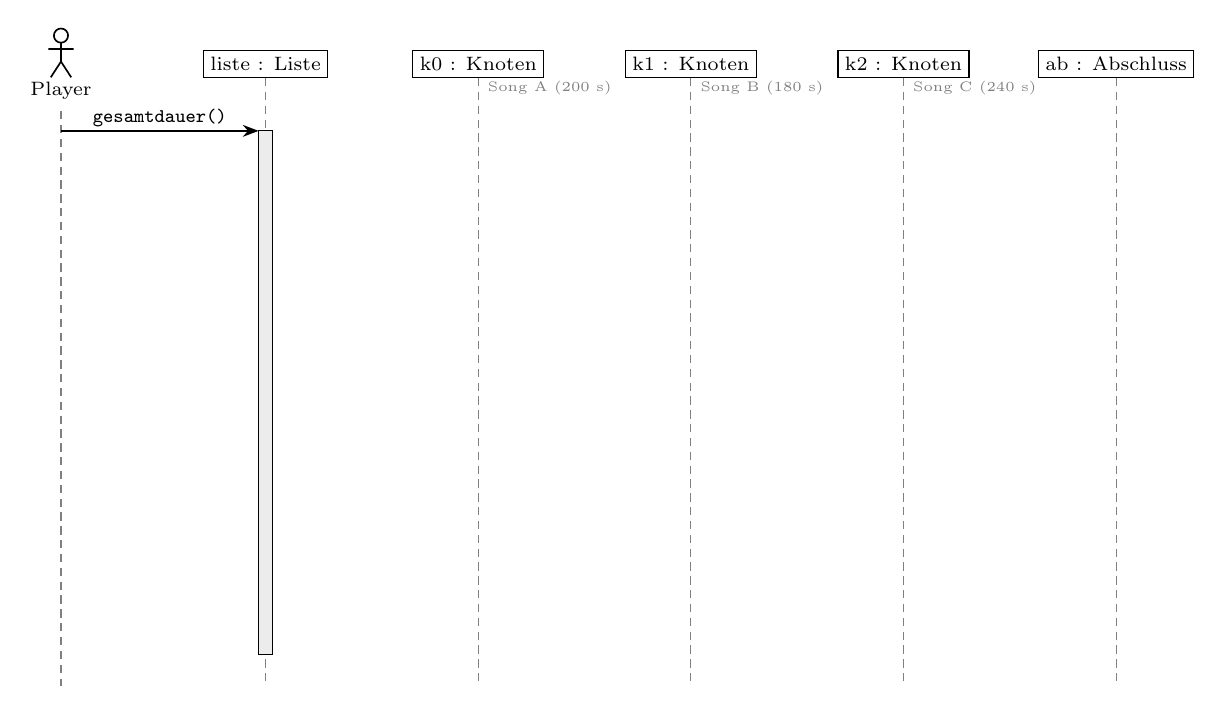
\begin{tikzpicture}[x=1cm,y=1cm]
\akteur{0.6}{0.45}{Player}
\draw[leben] (0.6,-0.6) -- (0.6,-7.9);
\foreach \name/\x/\txt/\inh in {li/3.2/liste : Liste/, k0/5.9/k0 : Knoten/Song A (200 s),
    k1/8.6/k1 : Knoten/Song B (180 s), k2/11.3/k2 : Knoten/Song C (240 s), ab/14.0/ab : Abschluss/} {
  \node[lebenslinie] (\name) at (\x,0) {\txt};
  \node[inhalt,anchor=north west] at ([xshift=0.8mm]\name.south) {\inh};
  \draw[leben] (\name.south) -- (\x,-7.9);
}
\aktiv{3.2}{-0.85}{-7.5}
\draw[aufruf] (0.6,-0.85) -- node[msg] {\code{gesamtdauer()}} ([xshift=-0.09cm]3.2,-0.85);
\loesungsteil{%
  \aktiv{5.9}{-1.6}{-6.75}
  \aktiv{8.6}{-2.35}{-6.0}
  \aktiv{11.3}{-3.1}{-5.25}
  \aktiv{14.0}{-3.85}{-4.5}
  \ruf{3.2}{5.9}{-1.6}{gesamtdauer()}
  \ruf{5.9}{8.6}{-2.35}{gesamtdauer()}
  \ruf{8.6}{11.3}{-3.1}{gesamtdauer()}
  \ruf{11.3}{14.0}{-3.85}{gesamtdauer()}
  \rueck{14.0}{11.3}{-4.5}{0}
  \rueck{11.3}{8.6}{-5.25}{240}
  \rueck{8.6}{5.9}{-6.0}{420}
  \rueck{5.9}{3.2}{-6.75}{620}
  \draw[rueckgabe] ([xshift=-0.09cm]3.2,-7.5) -- node[msg] {\code{620}} (0.6,-7.5);
  \node[notiz,anchor=west] at (11.45,-4.83) {0 + 240};
  \node[notiz,anchor=west] at (8.75,-5.58) {240 + 180};
  \node[notiz,anchor=west] at (6.05,-6.33) {420 + 200};
}
\end{tikzpicture}

% ---------------------------------------------------------------- 3 seq-entfernen
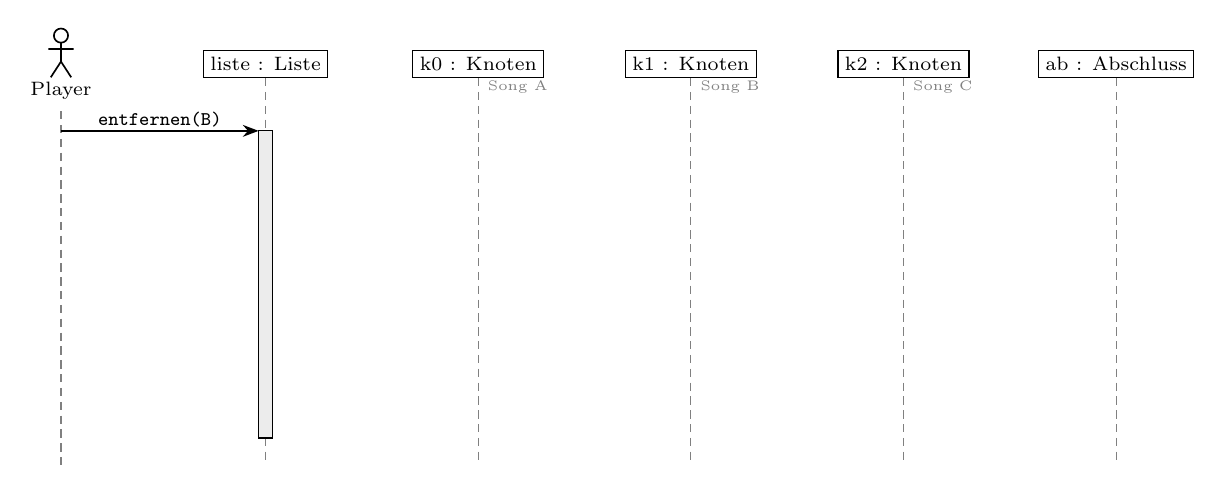
\begin{tikzpicture}[x=1cm,y=1cm]
\akteur{0.6}{0.45}{Player}
\draw[leben] (0.6,-0.6) -- (0.6,-5.1);
\foreach \name/\x/\txt/\inh in {li/3.2/liste : Liste/, k0/5.9/k0 : Knoten/Song A,
    k1/8.6/k1 : Knoten/Song B, k2/11.3/k2 : Knoten/Song C, ab/14.0/ab : Abschluss/} {
  \node[lebenslinie] (\name) at (\x,0) {\txt};
  \node[inhalt,anchor=north west] at ([xshift=0.8mm]\name.south) {\inh};
  \draw[leben] (\name.south) -- (\x,-5.1);
}
\aktiv{3.2}{-0.85}{-4.75}
\draw[aufruf] (0.6,-0.85) -- node[msg] {\code{entfernen(B)}} ([xshift=-0.09cm]3.2,-0.85);
\loesungsteil{%
  \aktiv{5.9}{-1.6}{-4.0}
  \aktiv{8.6}{-2.35}{-3.1}
  \ruf{3.2}{5.9}{-1.6}{entfernen(B)}
  \ruf{5.9}{8.6}{-2.35}{entfernen(B)}
  \node[notiz,anchor=west] at (6.05,-1.95) {A ist nicht B};
  \node[notiz,anchor=west] at (8.75,-2.7) {B gefunden};
  \rueck{8.6}{5.9}{-3.1}{k2}
  \node[notiz,anchor=west] at (6.05,-3.45) {nachfolger = k2};
  \rueck{5.9}{3.2}{-4.0}{k0}
  \node[notiz,anchor=west] at (3.35,-4.35) {anfang = k0};
  \draw[rueckgabe] ([xshift=-0.09cm]3.2,-4.75) -- node[msg] {\code{true}} (0.6,-4.75);
  \node[notiz,align=center] at (12.65,-3.0) {k2 und ab werden\\nicht aufgerufen};
}
\end{tikzpicture}

% ---------------------------------------------------------------- 4 seq-einfuegen (Trittbrett)
\begin{tikzpicture}[x=1cm,y=1cm]
\akteur{0.6}{0.45}{Player}
\draw[leben] (0.6,-0.6) -- (0.6,-6.5);
\foreach \name/\x/\txt/\inh in {li/3.0/liste : Liste/, k0/5.9/k0 : Knoten/Song A,
    k1/8.8/k1 : Knoten/Song B, ab/14.25/ab : Abschluss/} {
  \node[lebenslinie] (\name) at (\x,0) {\txt};
  \node[inhalt,anchor=north west] at ([xshift=0.8mm]\name.south) {\inh};
  \draw[leben] (\name.south) -- (\x,-6.5);
}
\node[lebenslinie] (neu) at (11.7,-3.3) {neu : Knoten};
\node[inhalt,anchor=north west] at ([xshift=0.8mm]neu.south) {Song X};
\draw[leben] (neu.south) -- (11.7,-6.5);
\aktiv{3.0}{-0.85}{-6.2}
\aktiv{5.9}{-1.45}{-5.5}
\aktiv{8.8}{-2.3}{-4.8}
\aktiv{11.7}{-4.0}{-4.3}
\draw[aufruf] (0.6,-0.85) -- node[msg] {\code{einfuegenAn(1, X)}} ([xshift=-0.09cm]3.0,-0.85);
\ruf{3.0}{5.9}{-1.45}{einfuegenAn(1, X)}
\node[notiz,anchor=west] at (6.05,-1.8) {[position ist nicht 0]};
\ruf{5.9}{8.8}{-2.3}{einfuegenAn(0, X)}
\node[notiz,anchor=west] at (8.95,-2.65) {[position ist 0]};
\draw[erzeugung] ([xshift=0.09cm]8.8,-3.3) -- node[msg] {«create»} (neu.west);
\ruf{8.8}{11.7}{-4.0}{setNachfolger(k1)}
\rueck{8.8}{5.9}{-4.8}{neu}
\node[notiz,anchor=west] at (6.05,-5.12) {nachfolger = neu};
\rueck{5.9}{3.0}{-5.5}{k0}
\node[notiz,anchor=west] at (3.15,-5.82) {anfang = k0};
\draw[rueckgabe] ([xshift=-0.09cm]3.0,-6.2) -- node[msg] {\code{true}} (0.6,-6.2);
\end{tikzpicture}

% ---------------------------------------------------------------- 5 doppelt
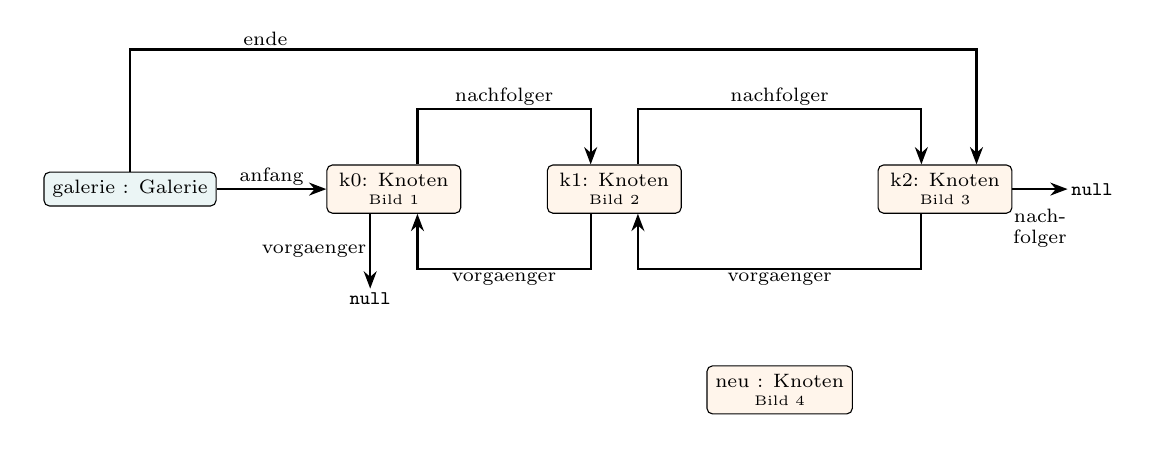
\begin{tikzpicture}[x=1cm,y=1cm]
\useasboundingbox (0,2.05) rectangle (14.2,-3.2);
\node[qobj] (ws) at (1.3,0) {galerie : Galerie};
\foreach \i/\x/\a in {0/4.65/1,1/7.45/2,2/11.65/3} {
  \node[obj] (k\i) at (\x,0) {k\i : Knoten\\[-0.5mm]{\tiny Bild \a}};
}
\node[obj] (neu) at (9.55,-2.55) {neu : Knoten\\[-0.5mm]{\tiny Bild 4}};
\draw[zeiger] (ws.east) -- node[rolle,above] {anfang} (k0.west);
\draw[zeiger] (ws.north) -- ++(0,1.55) -| ([xshift=4mm]k2.north) node[rolle,pos=0.08,above] {ende};
\foreach \i/\j in {0/1,1/2} {
  \draw[zeiger] ([xshift=3mm]k\i.north) -- ++(0,0.7) -| ([xshift=-3mm]k\j.north)
    node[rolle,pos=0.25,above] {nachfolger};
  \draw[zeiger] ([xshift=-3mm]k\j.south) -- ++(0,-0.7) -| ([xshift=3mm]k\i.south)
    node[rolle,pos=0.25,below] {vorgaenger};
}
\draw[zeiger] ([xshift=-3mm]k0.south) -- ++(0,-0.95) node[rolle,below,font=\scriptsize\ttfamily] {null}
  node[rolle,pos=0.5,left] {vorgaenger};
\draw[zeiger] (k2.east) -- ++(0.7,0) node[rolle,right,font=\scriptsize\ttfamily] {null}
  node[rolle,pos=0.5,below=2mm] {\shortstack{nach-\\folger}};
\loesungsteil{%
  \coordinate (x1) at ($([xshift=3mm]k1.north)!0.85!([xshift=-3mm]k2.north)+(0,0.7)$);
  \coordinate (x2) at ($([xshift=-3mm]k2.south)!0.75!([xshift=3mm]k1.south)+(0,-0.7)$);
  \foreach \p in {x1,x2} {
    \draw[very thick] ($(\p)+(-0.15,-0.15)$) -- ($(\p)+(0.15,0.15)$) ($(\p)+(-0.15,0.15)$) -- ($(\p)+(0.15,-0.15)$);
  }
  \draw[zeiger] (k1.east) -| ([xshift=-3mm]neu.north) node[rolle,pos=0.75,sloped,below] {nachfolger};
  \draw[zeiger] ([xshift=3mm]neu.north) |- (k2.west) node[rolle,pos=0.25,sloped,below] {nachfolger};
  \draw[zeiger] (neu.west) -| ([xshift=6mm]k1.south) node[rolle,pos=0.75,sloped,above] {vorgaenger};
  \draw[zeiger] ([xshift=-6mm]k2.south) |- (neu.east) node[rolle,pos=0.25,sloped,above] {vorgaenger};
}
\end{tikzpicture}

% ---------------------------------------------------------------- 6 baum (nur Lösung)
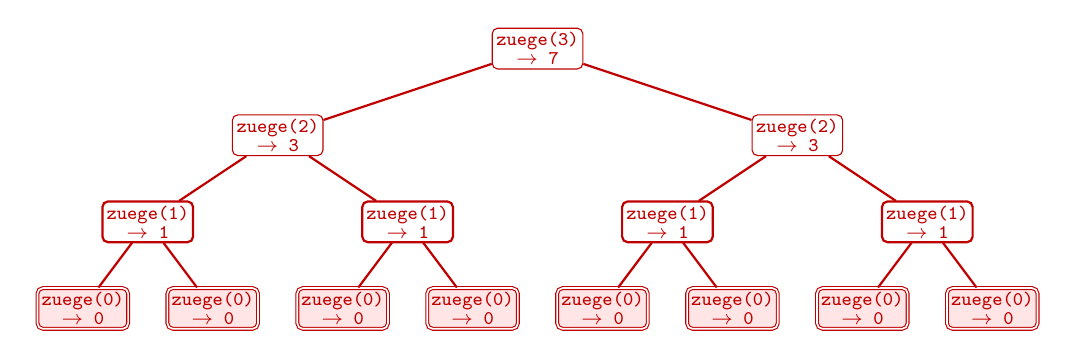
\begin{tikzpicture}[lsgbild,level distance=11mm,
  every node/.style={draw,rounded corners=2pt,fill=white,font=\scriptsize\ttfamily,inner sep=1.5pt,align=center},
  abbruch/.style={fill=red!10,double,double distance=0.6pt},
  edge from parent/.style={draw,thick},
  level 1/.style={sibling distance=66mm},
  level 2/.style={sibling distance=33mm},
  level 3/.style={sibling distance=16.5mm}]
\node {zuege(3)\\[-0.4mm]$\to$ 7}
  child {node {zuege(2)\\[-0.4mm]$\to$ 3}
    child {node {zuege(1)\\[-0.4mm]$\to$ 1}
      child {node[abbruch] {zuege(0)\\[-0.4mm]$\to$ 0}}
      child {node[abbruch] {zuege(0)\\[-0.4mm]$\to$ 0}}}
    child {node {zuege(1)\\[-0.4mm]$\to$ 1}
      child {node[abbruch] {zuege(0)\\[-0.4mm]$\to$ 0}}
      child {node[abbruch] {zuege(0)\\[-0.4mm]$\to$ 0}}}}
  child {node {zuege(2)\\[-0.4mm]$\to$ 3}
    child {node {zuege(1)\\[-0.4mm]$\to$ 1}
      child {node[abbruch] {zuege(0)\\[-0.4mm]$\to$ 0}}
      child {node[abbruch] {zuege(0)\\[-0.4mm]$\to$ 0}}}
    child {node {zuege(1)\\[-0.4mm]$\to$ 1}
      child {node[abbruch] {zuege(0)\\[-0.4mm]$\to$ 0}}
      child {node[abbruch] {zuege(0)\\[-0.4mm]$\to$ 0}}}};
\path ([xshift=-1mm]current bounding box.west) ([xshift=1mm]current bounding box.east);
\end{tikzpicture}

\end{document}
